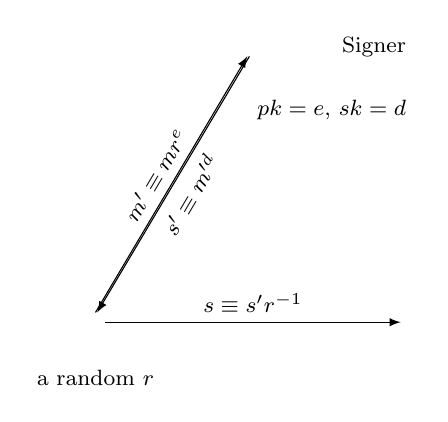
\begin{tikzpicture}[font=\footnotesize]
\node (A) at (0,0) {\Lisa};
\node (r) at (0,-0.7) {a random $r$};
\node (B) [right of = A, node distance = 4cm] {\Left\Bart};
\node (KDC) at (2,3.5) [rounded corners=1ex,minimum width=2cm,label distance=-1.5cm,label=right:Signer] {\Homer};
\node at (3,2.7) {$pk=e$, $sk = d$};  
\draw[-latex] (A) -- (B) node [midway,above] {$s \equiv s'r^{-1}$};
\draw[-latex] (A.90) -- (KDC.240) node [sloped,midway,above] {$m' \equiv mr^e$
};
\draw[-latex] (KDC.250) --  (A.80) node [sloped,midway,below] {$s' \equiv m'^d$};
%\draw[-latex] (KDC.320) to [bend left=40] node [sloped,midway,above] {$\mathsf{cert}_{C\to B}$} (B.70);
%\draw[-latex,dotted] (B.100) -- (KDC.290) node [sloped,midway,below] {Charlie knows $pk_B$.} node [sloped,midway,above] {Bob trusts Charlie.};
\end{tikzpicture}